%%%%%%%%%%%%%%%%%%%%%%%%%%%%%%%%%%%%%%%%%%%%%%%%%%%%%%%%%%%%%%%%%%%
%%%
%%% File ini ditujukan untuk menulis 
%%% Paper POMITS menggunakan LaTeX untuk program sarjana
%%% di Institut Teknologi Sepuluh Nopember, Surabaya.
%%%
%%% Komentar, saran, koreksi, modifikasi untuk file ini dipersilakan
%%%
%%% Didapat dari: Ahmad Zaki Al Muntazhar
%%% Matematika ITS 2019
%%% Revisi terahir oleh: Ahmad Hisbu Zakiyudin
%%% Matematika ITS 2020
%%% <azakiyudin1790@gmail.com>
%%% Revisi terakhir (Juni 2024): 
%%% 1. Penyesuaian Header (masih belum sama persis), 
%%% 2. Penyesuaian Penomoran Definisi, Teorema, Contoh, dan Persamaan (2022),
%%% 3. Penyempurnaan sesuai Format POMITS.
%%%
%%%%%%%%%%%%%%%%%%%%%%%%%%%%%%%%%%%%%%%%%%%%%%%%%%%%%%%%%%%%%%%%%%%%
\documentclass[journal]{IEEEtran}
% correct bad hyphenation here
\hyphenation{op-tical net-works semi-conduc-tor}
\usepackage{amssymb,amsmath,amsthm,graphicx}
\usepackage{caption,tabularx,multicol,multirow}
\usepackage{listings,color,booktabs}
\usepackage{float}
\usepackage{algpseudocode}
\usepackage{array}
\usepackage{tikz}
\usetikzlibrary{arrows.meta,positioning}
\usepackage{scrfontsizes}
\usepackage{afterpage}
\usepackage{subfig}
\usepackage{mathtools}
\usepackage{physics}
\usepackage[ruled,vlined]{algorithm2e}
\usepackage{algpseudocode}
\captionsetup[figure]{labelsep=period}
\captionsetup[figure]{name={Gambar}}

\captionsetup[table]{labelsep=newline}
\captionsetup[table]{name={Tabel}}
\tolerance=1
\emergencystretch=\maxdimen
\hyphenpenalty=10000
\hbadness=10000
\setlength{\parindent}{0.36cm}
\newenvironment{breakablealgorithm}
  {% \begin{breakablealgorithm}
   \begin{center}
     \refstepcounter{algorithm}% New algorithm
     \hrule height.8pt depth0pt \kern2pt% \@fs@pre for \@fs@ruled
     \renewcommand{\caption}[2][\relax]{% Make a new \caption
       {\raggedright\textbf{\fname@algorithm~\thealgorithm} ##2\par}%
       \ifx\relax##1\relax % #1 is \relax
         \addcontentsline{loa}{algorithm}{\protect\numberline{\thealgorithm}##2}%
       \else % #1 is not \relax
         \addcontentsline{loa}{algorithm}{\protect\numberline{\thealgorithm}##1}%
       \fi
       \kern2pt\hrule\kern2pt
     }
  }{% \end{breakablealgorithm}
     \kern2pt\hrule\relax% \@fs@post for \@fs@ruled
   \end{center}
  }


\newtheorem{defn}{Definisi}[section]
\newtheorem{teo}[defn]{Teorema}
\newtheorem{thm}{Teorema}
\newtheorem{lemma}{Lemma}
\newtheorem{lemmas}[defn]{Lemma}
\newtheorem{cor}[defn]{Akibat}
\newtheorem{asumsi}[defn]{Asumsi}
\theoremstyle{definition}
\newtheorem{con}{Contoh}[section]
\theoremstyle{definition}
\theoremstyle{plain}
\newtheorem{prop}{Proposisi}
\renewcommand{\proofname}{Bukti}
\renewcommand{\thedefn}{\arabic{section}.\arabic{defn}}
\renewcommand{\thecon}{\arabic{section}.\arabic{con}}

\newcommand{\normlp}[1]{\left\|#1\right\|_{L^p_{\lambda}(0,T;H)}}% Fungsi norm (||x||)
\newcommand{\R}{\mathbb{R}}
\renewcommand{\natural}{\mathbb{N}}
\newcommand{\Xpl}{X^R_{p,\lambda}}
\newcommand{\Xpls}{X^R_{p,\lambda^*}}
\newcommand{\qpl}{q^R_{p,\lambda}}
\newcommand{\qpls}{q^R_{p,\lambda^*}}
\newcommand{\katakunci}[1]{%
    \noindent\\
    \textit{\textbf{Kata Kunci---}}{\textbf{#1}}
}

%\renewcommand\thetheorem{\arabic{section}.\arabic{theorem}}
\renewcommand{\listfigurename}{\hfill\normalsize\textbf{DAFTAR GAMBAR}\hfill}
\renewcommand{\listtablename}{\hfill\normalsize\textbf{DAFTAR TABEL}\hfill}
\renewcommand{\contentsname}{\hfill\normalsize\textbf{DAFTAR ISI}\hfill}
\renewcommand{\refname}{}
\renewcommand{\arraystretch}{1.2}

\newcolumntype{L}[1]{>{\raggedright\let\newline\\\arraybackslash\hspace{0pt}}m{#1}}
\newcolumntype{C}[1]{>{\centering\let\newline\\\arraybackslash\hspace{0pt}}m{#1}}
\newcolumntype{R}[1]{>{\raggedleft\let\newline\\\arraybackslash\hspace{0pt}}m{#1}}

\definecolor{codegreen}{rgb}{0,0.6,0}
\definecolor{codegray}{rgb}{0.5,0.5,0.5}
\definecolor{codepurple}{rgb}{0.58,0,0.82}
\definecolor{ITSblue}{rgb}{0.08,0.38,0.74}

\lstdefinestyle{mypseudo}{ 
commentstyle=\bfseries,
keywordstyle=\bfseries,
breakatwhitespace=false,         
breaklines=true,                 
captionpos=b,                    
keepspaces=true,                  
showspaces=false,                
showstringspaces=false,
showtabs=false,
literate={\ \ }{{\ }}2
}
\lstset{basicstyle=\sffamily\scriptsize,style=mypseudo}
\def\abstractname{Abstrak}
%\renewcommand{\thetable}{\arabic{table}}

\begin{document}

    \title{\changefontsizes{24}OPTIMASI RANTAI PASOK KEDELAI NASIONAL MULTI-PERIODE \textit{MENGGUNAKAN ADAPTIVE LARGE NEIGHBORHOOD SEARCH}\\ \vspace{12pt}}

    \author{\changefontsizes{11}Alief Randiansyah Pradanaputra, Imam Mukhlash, Siti Komsiyah\\
    Departemen Matematika\\Institut Teknologi Sepuluh Nopember (ITS)\\
    Jl. Arief Rahman Hakim, Surabaya 60111 Indonesia\\
    \textit{e-mail} : aliefrandiansyahp@gmail.com, imamm@matematika.its.ac.id, citie\_math@binus.ac.id\\ \vspace{-1em}}
    \markboth{\small JURNAL TEKNIK ITS Vol. X, No. Y, (TAHUN) ISSN: 2337-3539 (2301-9271 Print)}{}

     \maketitle

    \begin{abstract}
Kedelai merupakan komoditas pangan strategis bagi Indonesia, namun ketergantungan impor yang mencapai lebih dari 85 persen kebutuhan nasional menjadikan alokasi pasokan dari sumber lokal dan impor sebagai persoalan kritis ketahanan pangan. Distribusi volume impor melalui pelabuhan tertentu ke 38 provinsi dengan tingkat kebutuhan yang berbeda-beda memerlukan perencanaan yang mempertimbangkan biaya, kapasitas, dan batas kebijakan secara simultan. Penelitian ini bertujuan mengoptimalkan alokasi pasokan kedelai nasional multi-periode melalui pendekatan metaheuristik yang mampu menangani skala permasalahan praktis. Masalah diformulasikan sebagai model \textit{Mixed Integer Linear Programming} (MILP) yang mencakup produksi lokal, impor, distribusi pelabuhan, transfer antarprovinsi, inventori, dan \textit{shortage} selama 12 bulan. Karena kombinasi variabel kontinu dan logika biner membuat penyelesaian eksak tidak praktis, penelitian ini mengimplementasikan \textit{Adaptive Large Neighborhood Search} (ALNS) dengan representasi solusi berbasis tensor dan tiga konfigurasi \textit{local intensification}: ALNS-TS, ALNS-PRS \textit{adapted}, dan ALNS-\textit{only}. Evaluasi \textit{baseline} pada 50 \textit{seed} menunjukkan ALNS-PRS \textit{adapted} sebagai konfigurasi terbaik dengan \textit{shortage} rata-rata mendekati nol. Analisis 16 skenario \textit{what-if} mengungkapkan bahwa sistem paling rentan terhadap penurunan kapasitas pelabuhan dan kenaikan permintaan, sementara pengetatan batas ketergantungan impor di bawah 90 persen tidak realistis tanpa peningkatan produksi lokal. Penelitian ini telah berhasil mengembangkan model optimasi alokasi pasokan kedelai nasional yang mampu menangani persoalan multi-periode berskala nasional dan memberikan rekomendasi kebijakan berbasis skenario.
\end{abstract}

    \katakunci{\small Kedelai; \textit{Inventory-Transportation Problem}; ALNS; MILP; Supply Chain.}

    \IEEEpeerreviewmaketitle

     \section{PENDAHULUAN}
     \normalsize \IEEEPARstart{K}{EDELAI} merupakan komoditas pangan penting bagi Indonesia karena menjadi bahan utama tempe, tahu, kecap, dan berbagai produk pangan lain. Permintaan nasional berada pada kisaran 2,5--3 juta ton per tahun, sedangkan produksi domestik masih jauh lebih rendah daripada kebutuhan. Produksi domestik tahun 2023 hanya sekitar 349,10 ribu ton atau 13,14\% dari kebutuhan 2,66 juta ton, sehingga sebagian besar kebutuhan dipenuhi melalui impor \cite{kementan2024kedelai,pusdatin2024konsumsi}. Kondisi ini meningkatkan paparan terhadap volatilitas harga global, nilai tukar, dan ketersediaan pasokan eksternal.

     Persoalan kedelai tidak hanya terletak pada kecukupan volume nasional. Berdasarkan Survei Pola Distribusi Kedelai BPS 2023, 81,48\% provinsi yang tercatat mengalami defisit antara produksi lokal dan kebutuhan wilayahnya \cite{bps2023distribusi}. Pada saat yang sama, rantai distribusi kedelai lokal dan impor memiliki struktur berbeda; kedelai lokal melalui rantai multi-aktor, sedangkan kedelai impor umumnya masuk melalui importir lalu pedagang besar atau distributor \cite{cips2023logistics}. Karena itu, keputusan alokasi perlu mempertimbangkan sumber pasokan, pelabuhan masuk, provinsi tujuan, transfer antarprovinsi, dan inventori bulanan secara simultan.

     Penelitian sebelumnya telah memodelkan rantai pasok kedelai dengan pendekatan optimasi, misalnya desain rantai pasok kedelai berkelanjutan dan perencanaan taktis berbasis program stokastik \cite{SHARIFI2023,reis2023stochastic}. Namun, konteks ketahanan pangan nasional Indonesia membutuhkan formulasi yang memasukkan batas kebijakan seperti ketergantungan impor, penyerapan produksi lokal, inventori minimum, dan mekanisme redistribusi stok antarprovinsi. Model MILP dengan variabel kontinu dan logika biner dapat menghadapi pertumbuhan ruang pencarian yang besar pada penyelesaian eksak \cite{ntnu_milp}, sedangkan model jaringan rantai pasok berskala besar sering tidak praktis diselesaikan hingga optimal oleh \textit{solver} umum \cite{ESKANDARPOUR2017lns_supply}.

     Kontribusi artikel ini adalah menyusun formulasi MILP multi-periode untuk alokasi rantai pasok kedelai nasional sebagai \textit{Inventory-Transportation Problem} (ITP), mengimplementasikan ALNS dengan solusi awal berbasis data historis dan \textit{feasibility repair}, mengevaluasi tiga konfigurasi ALNS, serta melakukan analisis 16 skenario deterministik untuk membaca sensitivitas terhadap harga, kapasitas impor, kapasitas pelabuhan, permintaan, dan batas ketergantungan impor.

    \section{METODE PENELITIAN}
    \subsection{Ruang Lingkup dan Data}
    Sistem yang dimodelkan mencakup 38 provinsi konsumen, 20 sentra produksi lokal, 7 \textit{origin} impor, 11 pelabuhan impor, dan horizon 12 bulan. Pelabuhan diperlakukan sebagai titik \textit{throughput}; seluruh impor yang masuk pada bulan $t$ harus keluar sebagai distribusi ke provinsi pada bulan yang sama. Dengan asumsi ini, pelabuhan tidak menyimpan inventori, melainkan hanya menjadi penghubung antara keputusan pembelian impor dan keputusan distribusi ke provinsi.

    \begin{figure*}[t]
    \centering
    \resizebox{0.95\textwidth}{!}{%
    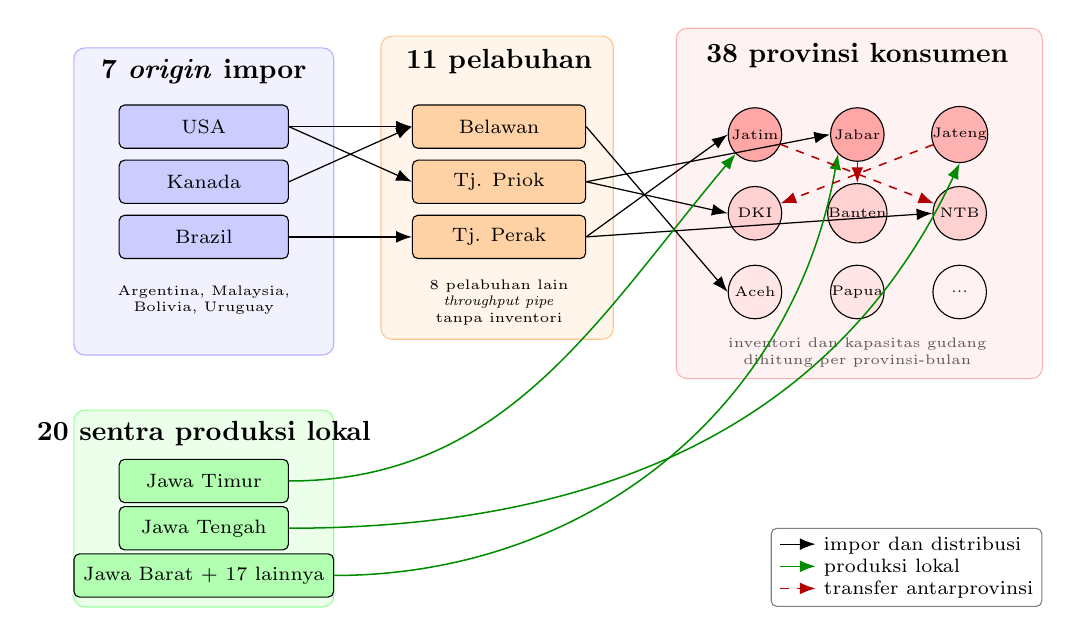
\begin{tikzpicture}[
        font=\scriptsize,
        source/.style={rectangle, draw=black, fill=blue!20, rounded corners=2pt, minimum width=2.15cm, minimum height=0.55cm, align=center},
        port/.style={rectangle, draw=black, fill=orange!35, rounded corners=2pt, minimum width=2.20cm, minimum height=0.55cm, align=center},
        producer/.style={rectangle, draw=black, fill=green!30, rounded corners=2pt, minimum width=2.15cm, minimum height=0.55cm, align=center},
        province/.style={circle, draw=black, fill=red!18, minimum size=0.68cm, inner sep=0pt, align=center, font=\tiny},
        arrow/.style={-{Latex[length=2mm]}, line width=0.45pt},
        localarrow/.style={-{Latex[length=2mm]}, line width=0.55pt, draw=green!55!black},
        transferarrow/.style={-{Latex[length=2mm]}, line width=0.55pt, draw=red!70!black, dashed}
    ]
    \draw[rounded corners=4pt, fill=blue!5, draw=blue!30] (-0.55,0.75) rectangle (2.75,4.65);
    \draw[rounded corners=4pt, fill=orange!8, draw=orange!45] (3.35,0.95) rectangle (6.30,4.80);
    \draw[rounded corners=4pt, fill=red!5, draw=red!30] (7.10,0.45) rectangle (11.75,4.90);
    \draw[rounded corners=4pt, fill=green!8, draw=green!40] (-0.55,-2.45) rectangle (2.75,0.05);

    \node[font=\bfseries] at (1.10,4.35) {7 \textit{origin} impor};
    \node[source] (usa) at (1.10,3.65) {USA};
    \node[source] (can) at (1.10,2.95) {Kanada};
    \node[source] (bra) at (1.10,2.25) {Brazil};
    \node[align=center, font=\tiny] at (1.10,1.45) {Argentina, Malaysia,\\Bolivia, Uruguay};

    \node[font=\bfseries] at (4.85,4.48) {11 pelabuhan};
    \node[port] (bel) at (4.85,3.65) {Belawan};
    \node[port] (priok) at (4.85,2.95) {Tj. Priok};
    \node[port] (perak) at (4.85,2.25) {Tj. Perak};
    \node[font=\tiny, align=center] at (4.85,1.42) {8 pelabuhan lain\\\textit{throughput pipe}\\tanpa inventori};

    \node[font=\bfseries] at (9.40,4.55) {38 provinsi konsumen};
    \node[province, fill=red!35] (jatim) at (8.10,3.55) {Jatim};
    \node[province, fill=red!35] (jabar) at (9.40,3.55) {Jabar};
    \node[province, fill=red!30] (jateng) at (10.70,3.55) {Jateng};
    \node[province] (dki) at (8.10,2.55) {DKI};
    \node[province] (banten) at (9.40,2.55) {Banten};
    \node[province] (ntb) at (10.70,2.55) {NTB};
    \node[province, fill=red!10] (aceh) at (8.10,1.55) {Aceh};
    \node[province, fill=red!10] (papua) at (9.40,1.55) {Papua};
    \node[province, fill=red!5] (other) at (10.70,1.55) {...};
    \node[font=\tiny, align=center, text=gray!70!black] at (9.40,0.78) {inventori dan kapasitas gudang\\dihitung per provinsi-bulan};

    \node[font=\bfseries] at (1.10,-0.25) {20 sentra produksi lokal};
    \node[producer] (prod1) at (1.10,-0.85) {Jawa Timur};
    \node[producer] (prod2) at (1.10,-1.45) {Jawa Tengah};
    \node[producer] (prod3) at (1.10,-2.05) {Jawa Barat + 17 lainnya};

    \draw[arrow] (usa.east) -- (bel.west);
    \draw[arrow] (usa.east) -- (priok.west);
    \draw[arrow] (can.east) -- (bel.west);
    \draw[arrow] (bra.east) -- (perak.west);
    \draw[arrow] (bel.east) -- (aceh.west);
    \draw[arrow] (priok.east) -- (jabar.west);
    \draw[arrow] (priok.east) -- (dki.west);
    \draw[arrow] (perak.east) -- (jatim.west);
    \draw[arrow] (perak.east) -- (ntb.west);

    \draw[localarrow] (prod1.east) to[out=0,in=230] (jatim.south west);
    \draw[localarrow] (prod2.east) to[out=0,in=245] (jateng.south);
    \draw[localarrow] (prod3.east) to[out=0,in=260] (jabar.south west);

    \draw[transferarrow] (jatim) -- (ntb);
    \draw[transferarrow] (jateng) -- (dki);
    \draw[transferarrow] (jabar) -- (banten);

    \node[draw=gray, fill=white, rounded corners=2pt, align=left, anchor=south east, inner sep=3pt] at (11.75,-2.45) {
        \tikz{\draw[arrow] (0,0) -- (0.45,0);} impor dan distribusi\\
        \tikz{\draw[localarrow] (0,0) -- (0.45,0);} produksi lokal\\
        \tikz{\draw[transferarrow] (0,0) -- (0.45,0);} transfer antarprovinsi
    };
    \end{tikzpicture}%
    }
    \caption{Struktur jaringan rantai pasok kedelai nasional yang digunakan: 7 \textit{origin} impor, 11 pelabuhan transit (\textit{throughput pipe}), 20 sentra produksi lokal, dan 38 provinsi konsumen dengan mekanisme transfer antar-wilayah. Pelabuhan tidak menyimpan inventori; seluruh impor yang masuk langsung didistribusikan pada periode yang sama.}
    \label{fig:rantai_pasok_paper}
    \end{figure*}

    \begin{table}[H]
    \centering
    \caption{Dimensi utama model}
    \label{tab:dimensi}
    \begin{tabular}{lr}
    \toprule
    \textbf{Komponen} & \textbf{Jumlah} \\
    \midrule
    Provinsi konsumen & 38 \\
    Sentra produksi lokal & 20 \\
    Origin impor & 7 \\
    Pelabuhan impor & 11 \\
    Periode perencanaan & 12 bulan \\
    \bottomrule
    \end{tabular}
    \end{table}

    Data sekunder dikumpulkan dari sumber nasional dan diubah menjadi parameter numerik yang konsisten. Permintaan bulanan provinsi dibaca dari proyeksi neraca kedelai 2024. Produksi lokal menggunakan data BPS tahunan yang didistribusikan ke bulan perencanaan menggunakan pola musim panen. Data impor menurut negara asal, data impor menurut pelabuhan, dan data historis negara-pelabuhan-bulan digunakan untuk membentuk kapasitas \textit{origin} impor, kapasitas \textit{throughput} pelabuhan, harga CIF, dan pola solusi awal. Koordinat provinsi dan pelabuhan digunakan untuk membangun biaya transportasi berbasis jarak, sedangkan kluster wilayah digunakan untuk membedakan karakter biaya antarpulau. Struktur model mengikuti gagasan masalah inventori-transportasi multi-periode pada literatur ITP \cite{SAINATHUNI2014690,DE2020107566}.

    Hasil pra-pemrosesan data dinyatakan dalam bentuk \textit{array} parameter. Permintaan menjadi matriks $D_{i,t}$, produksi lokal menjadi $Cap^{PROD}_{k,t}$, kapasitas \textit{origin} impor menjadi $Cap^{IMP}_{s,t}$, kapasitas pelabuhan menjadi $Cap^{PORT}_{h,t}$, dan kapasitas gudang provinsi menjadi $Cap^{STOR}_{i}$. Biaya dikonstruksi sebagai biaya produksi dan pengiriman lokal $(C^{PROD}_{k},C^{SHIP}_{k,i})$, biaya pembelian impor $C^{PURCH}_{s}$, biaya distribusi pelabuhan $C^{DIST}_{h,i}$, biaya transfer antarprovinsi $C^{TRANS}_{i,j}$, biaya simpan $H^{PROV}_{i}$, dan biaya aktivasi kontrak impor $F^{ACT}_{s}$. Bentuk \textit{array} tersebut membuat seluruh keputusan dapat dibaca sebagai aliran pada indeks sumber, tujuan, dan waktu.

    Ringkasan hasil transformasi data yang digunakan oleh model ditunjukkan pada Tabel \ref{tab:parameter_model}. Tabel ini penting karena model tidak bekerja langsung dengan \textit{file} mentah, tetapi dengan parameter numerik yang indeksnya sudah diselaraskan. Misalnya, data permintaan provinsi harus memiliki indeks provinsi dan bulan yang sama dengan data alokasi, sedangkan kapasitas pelabuhan harus memiliki indeks pelabuhan dan bulan yang sama dengan aliran impor yang masuk. Dengan cara ini, setiap operasi pada model dapat dicek kembali terhadap dimensi parameter yang sesuai.

    \begin{table}[H]
    \centering
    \caption{Parameter utama hasil pra-pemrosesan data}
    \label{tab:parameter_model}
    \resizebox{\columnwidth}{!}{%
    \begin{tabular}{lll}
    \toprule
    \textbf{Parameter} & \textbf{Dimensi} & \textbf{Makna operasional} \\
    \midrule
    $D_{i,t}$ & $38 \times 12$ & permintaan provinsi per bulan \\
    $Cap^{PROD}_{k,t}$ & $20 \times 12$ & kapasitas produksi lokal musiman \\
    $Cap^{IMP}_{s,t}$ & $7 \times 12$ & kapasitas \textit{origin} impor per bulan \\
    $Cap^{PORT}_{h,t}$ & $11 \times 12$ & kapasitas \textit{throughput} pelabuhan \\
    $HIST\_IMPORT_{s,h,t}$ & $7 \times 11 \times 12$ & pola historis impor awal \\
    $C^{SHIP},C^{DIST},C^{TRANS}$ & matriks biaya & biaya pengiriman dan transfer \\
    \bottomrule
    \end{tabular}}
    \end{table}

    \subsection{Formulasi Model}
    Keputusan utama adalah aliran produksi lokal $x^{loc}_{k,i,t}$, impor reguler $x^{imp}_{s,h,t}$, distribusi pelabuhan $x^{dist}_{h,i,t}$, dan transfer antarprovinsi $x^{trns}_{i,j,t}$. Variabel turunan meliputi inventori $inv_{i,t}$, \textit{shortage} $sh_{i,t}$, aktivasi impor $y_{s,t}$, status stok aman $safe_{i,t}$, dan kelayakan transfer keluar $w_{i,t}$. Secara implementatif, satu solusi disimpan sebagai kumpulan \textit{tensor} aliran $X^{loc}$, $X^{imp}$, $X^{dist}$, dan $X^{trns}$, kemudian $inv$, $sh$, $safe$, $w$, dan $y$ dihitung ulang setiap kali aliran berubah.

    Notasi yang digunakan pada formulasi MILP diringkas pada Tabel \ref{tab:notasi_milp_paper}. Tabel ini hanya memuat simbol yang muncul langsung pada fungsi objektif, kendala, dan metrik strategis, sehingga pembaca dapat mengikuti persamaan tanpa harus kembali ke daftar simbol naskah utama.

    \begin{table}[H]
    \centering
    \caption{Notasi utama pada formulasi MILP}
    \label{tab:notasi_milp_paper}
    \scriptsize
    \begin{tabularx}{\columnwidth}{@{}p{0.30\columnwidth}X@{}}
    \toprule
    \textbf{Notasi} & \textbf{Arti} \\
    \midrule
    \multicolumn{2}{@{}l}{Indeks} \\
    $i,j\in I$ & provinsi konsumen; $i$ juga menjadi asal dan $j$ menjadi tujuan pada transfer antarprovinsi \\
    $k\in K$ & sentra produksi lokal \\
    $s\in S$ & \textit{origin} impor \\
    $h\in H$ & pelabuhan impor sebagai \textit{throughput pipe} \\
    $t\in T$ & bulan perencanaan \\
    $n\in\{1,2,3\}$ & jeda bulan untuk mengecek stok aman tiga bulan sebelumnya \\
    \addlinespace[1mm]
    \multicolumn{2}{@{}l}{Variabel keputusan dan turunan} \\
    $x^{loc}_{k,i,t}$ & aliran kedelai lokal dari sentra $k$ ke provinsi $i$ pada bulan $t$ \\
    $x^{imp}_{s,h,t}$ & impor reguler dari \textit{origin} $s$ ke pelabuhan $h$ pada bulan $t$ \\
    $x^{dist}_{h,i,t}$ & distribusi dari pelabuhan $h$ ke provinsi $i$ pada bulan $t$ \\
    $x^{trns}_{i,j,t}$ & transfer kedelai dari provinsi $i$ ke provinsi $j$ pada bulan $t$ \\
    $inv_{i,t}$, $sh_{i,t}$ & inventori akhir dan \textit{shortage} provinsi $i$ pada bulan $t$ \\
    $y_{s,t}$, $safe_{i,t}$, $w_{i,t}$ & indikator aktivasi impor, status stok aman, dan izin transfer keluar \\
    \addlinespace[1mm]
    \multicolumn{2}{@{}l}{Parameter fisik dan biaya} \\
    $D_{i,t}$, $SS_i$, $M$ & permintaan, ambang stok aman, dan konstanta besar untuk kendala logika \\
    $Cap^{PROD}_{k,t}$, $Cap^{IMP}_{s,t}$ & kapasitas produksi lokal dan kapasitas \textit{origin} impor \\
    $Cap^{PORT}_{h,t}$, $Cap^{STOR}_{i}$ & kapasitas pelabuhan dan kapasitas penyimpanan provinsi \\
    $C^{PROD}_{k}$, $C^{SHIP}_{k,i}$ & biaya produksi lokal dan biaya pengiriman lokal \\
    $C^{PURCH}_{s}$, $C^{DIST}_{h,i}$ & biaya pembelian impor dan distribusi dari pelabuhan \\
    $C^{TRANS}_{i,j}$, $H^{PROV}_{i}$, $F^{ACT}_{s}$ & biaya transfer, biaya simpan provinsi, dan biaya aktivasi impor \\
    \addlinespace[1mm]
    \multicolumn{2}{@{}l}{Metrik dan target strategis} \\
    $Z_{cost}$ & total biaya fisik rantai pasok yang diminimalkan \\
    $Q^{imp}$, $Q^{loc}$ & total impor reguler dan total serapan produksi lokal \\
    $\epsilon_1,\epsilon_2,\epsilon_3,\epsilon_4$ & batas \textit{shortage}, batas \textit{import dependency}, minimum serapan lokal, dan lantai inventori \\
    \bottomrule
    \end{tabularx}
    \end{table}

    Tujuan utama model adalah meminimalkan total biaya rantai pasok $Z_{cost}$:
    \begin{align}
    \min Z_{cost} =
    &\sum_{t,k,i} (C^{PROD}_{k}+C^{SHIP}_{k,i})x^{loc}_{k,i,t}
    + \sum_{t,s,h} C^{PURCH}_{s}x^{imp}_{s,h,t} \nonumber\\
    &+ \sum_{t,h,i} C^{DIST}_{h,i}x^{dist}_{h,i,t}
    + \sum_{t,i,j} C^{TRANS}_{i,j}x^{trns}_{i,j,t} \nonumber\\
    &+ \sum_{t,i} H^{PROV}_{i}inv_{i,t}
    + \sum_{t,s}F^{ACT}_{s}y_{s,t}.
    \label{eq:objective}
    \end{align}

    Keseimbangan inventori provinsi, keseimbangan pelabuhan, dan kapasitas utama ditulis sebagai:
    \begin{align}
    inv_{i,t} =&\ inv_{i,t-1}+\sum_k x^{loc}_{k,i,t}
    +\sum_h x^{dist}_{h,i,t}+\sum_j x^{trns}_{j,i,t} \nonumber\\
    &-\sum_j x^{trns}_{i,j,t}-D_{i,t}+sh_{i,t}, \quad \forall i,t, \label{eq:balance}\\
    \sum_i x^{dist}_{h,i,t} &= \sum_s x^{imp}_{s,h,t}, \quad \forall h,t, \label{eq:port}\\
    \sum_i x^{loc}_{k,i,t} &\leq Cap^{PROD}_{k,t}, \quad \forall k,t, \\
    \sum_s x^{imp}_{s,h,t} &\leq Cap^{PORT}_{h,t}, \quad \forall h,t, \\
    \sum_h x^{imp}_{s,h,t} &\leq Cap^{IMP}_{s,t}, \quad \forall s,t, \\
    inv_{i,t} &\leq Cap^{STOR}_{i}, \quad \forall i,t.
    \end{align}

    Aktivasi kontrak impor dan aturan transfer antarprovinsi ditulis sebagai kendala logika berbasis variabel biner:
    \begin{align}
    \sum_h x^{imp}_{s,h,t} &\leq M y_{s,t}, \quad \forall s,t, \\
    inv_{i,t} &\geq SS_i safe_{i,t}, \quad \forall i,t, \\
    inv_{i,t} &\leq SS_i-1+M safe_{i,t}, \quad \forall i,t, \\
    w_{i,t} &\leq safe_{i,t-n}, \quad \forall i,t\geq4,n=1,2,3, \\
    w_{i,t} &\geq \sum_{n=1}^{3}safe_{i,t-n}-2, \quad \forall i,t\geq4, \\
    \sum_j x^{trns}_{i,j,t} &\leq Mw_{i,t}, \quad \forall i,t.
    \end{align}
    Kendala pertama memastikan biaya aktivasi dikenakan ketika suatu \textit{origin} impor digunakan. Kendala berikutnya mendefinisikan status stok aman berdasarkan ambang $SS_i$, sedangkan kendala terakhir menyatakan bahwa provinsi hanya boleh mengirim transfer keluar setelah memenuhi kondisi stok aman pada tiga bulan sebelumnya.

    Target strategis ditangani melalui pendekatan $\epsilon$-\textit{constraint} dan penalti \textit{normalized} AUGMECON \cite{MAVROTAS_EPSILON}. Dengan
    \begin{align}
    Q^{imp}=\sum_{t,s,h}x^{imp}_{s,h,t}, \qquad
    Q^{loc}=\sum_{t,k,i}x^{loc}_{k,i,t},
    \end{align}
    target strategisnya adalah:
    \begin{align}
    \sum_{t,i} sh_{i,t} &\leq \epsilon_1, \\
    \frac{Q^{imp}}{Q^{imp}+Q^{loc}} &\leq \epsilon_2, \\
    Q^{loc} &\geq \epsilon_3, \\
    inv_{i,t} &\geq \epsilon_4D_{i,t}, \quad \forall i,t.
    \end{align}
    Nilai dasar yang digunakan adalah $\epsilon_1=0$, $\epsilon_2=0,90$, $\epsilon_3$ dikunci dari total produksi lokal solusi awal, dan $\epsilon_4=0,10$ dari permintaan bulanan. \textit{Service rate} dihitung sebagai $1-\sum_{i,t}sh_{i,t}/\sum_{i,t}D_{i,t}$, sedangkan \textit{import dependency} dihitung sebagai $Q^{imp}/(Q^{imp}+Q^{loc})$. Jika suatu target strategis tidak terpenuhi, besar pelanggaran dimasukkan sebagai penalti pada fungsi objektif sehingga pencarian tetap dapat berjalan pada kandidat yang belum sepenuhnya memenuhi seluruh target, tetapi diarahkan menuju solusi yang lebih layak.

    \subsection{Kerangka ALNS dan Eksperimen}
    ALNS bekerja pada representasi solusi berbasis \textit{tensor} aliran, bukan rute tunggal. Solusi awal dibentuk dengan \textit{historical seeding}: aliran impor $x^{imp}_{s,h,t}$ mengikuti data historis negara-pelabuhan-bulan setelah dibatasi oleh kapasitas pelabuhan, produksi lokal awal diarahkan terlebih dahulu ke provinsi produsennya, lalu aliran yang masuk pelabuhan didistribusikan ke provinsi menurut kebutuhan dengan prioritas biaya distribusi termurah. Tahap ini menghasilkan solusi awal yang sudah mengikuti pola data aktual, bukan solusi acak. Hubungan antara \textit{problem instance}, \textit{state} solusi, dan siklus perubahan kandidat ALNS diringkas pada Gambar \ref{fig:problem_state_alns_flow}.

    \begin{figure*}[t]
    \centering
    \resizebox{0.98\textwidth}{!}{%
    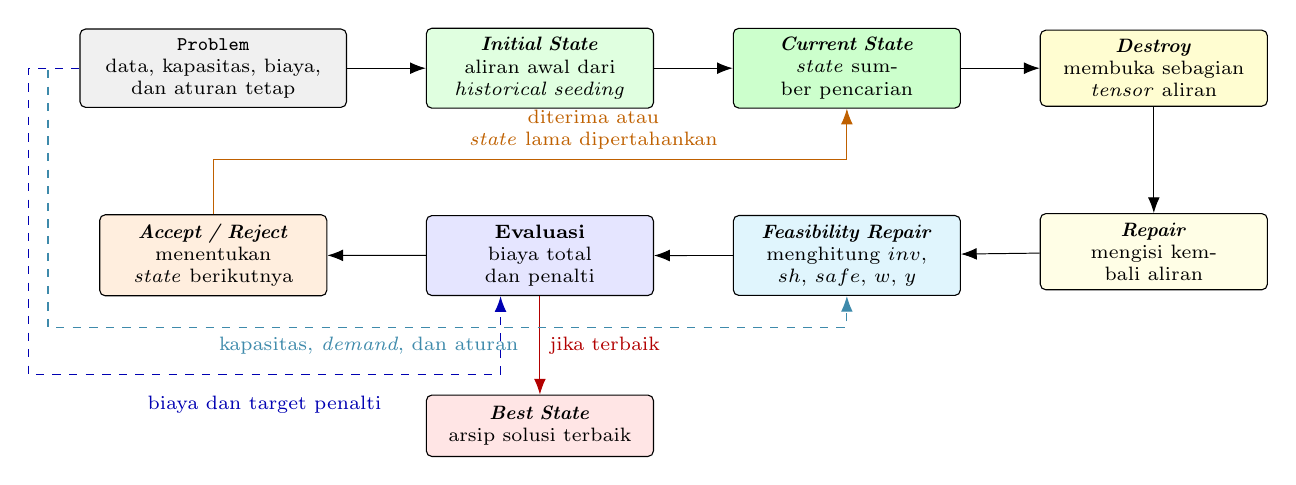
\begin{tikzpicture}[
        node distance=1.35cm and 1.0cm,
        box/.style={
            rectangle,
            draw=black,
            rounded corners=2pt,
            align=center,
            minimum width=2.75cm,
            minimum height=0.78cm,
            font=\scriptsize,
            text width=2.65cm
        },
        widebox/.style={
            rectangle,
            draw=black,
            rounded corners=2pt,
            align=center,
            minimum width=3.25cm,
            minimum height=0.82cm,
            font=\scriptsize,
            text width=3.15cm
        },
        arrow/.style={-{Latex[length=2mm]}, line width=0.35pt},
        rulearrow/.style={-{Latex[length=2mm]}, dashed, line width=0.45pt}
    ]
    \node[widebox, fill=gray!12] (problem) {\textbf{\texttt{Problem}}\\data, kapasitas, biaya, dan aturan tetap};
    \node[box, fill=green!12, right=of problem] (initial) {\textbf{\textit{Initial State}}\\aliran awal dari \textit{historical seeding}};
    \node[box, fill=green!20, right=of initial] (current) {\textbf{\textit{Current State}}\\\textit{state} sumber pencarian};
    \node[box, fill=yellow!18, right=of current] (destroy) {\textbf{\textit{Destroy}}\\membuka sebagian \textit{tensor} aliran};

    \node[box, fill=yellow!10, below=of destroy] (repair) {\textbf{\textit{Repair}}\\mengisi kembali aliran};
    \node[box, fill=cyan!12, below=of current] (feas) {\textbf{\textit{Feasibility Repair}}\\menghitung $inv$, $sh$, $safe$, $w$, $y$};
    \node[box, fill=blue!10, below=of initial] (eval) {\textbf{Evaluasi}\\biaya total dan penalti};
    \node[box, fill=orange!13, below=of problem] (accept) {\textbf{\textit{Accept / Reject}}\\menentukan \textit{state} berikutnya};
    \node[box, fill=red!10, below=1.25cm of eval] (best) {\textbf{\textit{Best State}}\\arsip solusi terbaik};

    \draw[arrow] (problem) -- (initial);
    \draw[arrow] (initial) -- (current);
    \draw[arrow] (current) -- (destroy);
    \draw[arrow] (destroy) -- (repair);
    \draw[arrow] (repair) -- (feas);
    \draw[arrow] (feas) -- (eval);
    \draw[arrow] (eval) -- (accept);
    \draw[arrow, draw=orange!75!black] (accept.north) -- ++(0,0.7) -| node[pos=0.3, above, align=center, font=\scriptsize, text=orange!75!black] {diterima atau\\\textit{state} lama dipertahankan} (current.south);
    \draw[arrow, draw=red!70!black] (eval) -- node[right, font=\scriptsize, text=red!70!black] {jika terbaik} (best);

    \draw[rulearrow, draw=cyan!65!black] (problem.west) -- ++(-0.4,0) |- node[pos=0.75, below, xshift=-1cm, font=\scriptsize, text=cyan!65!black] {kapasitas, \textit{demand}, dan aturan} ([yshift=-0.4cm]feas.south) -- (feas.south);
    \draw[rulearrow, draw=blue!70!black] (problem.west) -- ++(-0.65,0) |- node[pos=0.75, below, yshift=-0.15cm, font=\scriptsize, text=blue!70!black] {biaya dan target penalti} ([xshift=-0.5cm, yshift=-1.0cm]eval.south) -- ([xshift=-0.5cm]eval.south);
    \end{tikzpicture}%
    }
    \caption{Alur hubungan \textit{problem instance}, \textit{state}, dan siklus perubahan solusi pada ALNS.}
    \label{fig:problem_state_alns_flow}
    \end{figure*}

    Pada setiap iterasi, ALNS memilih satu operator \textit{destroy} dan satu operator \textit{repair} dengan mekanisme \textit{roulette wheel} berdasarkan bobot adaptif. Operator \textit{destroy} membuka sebagian aliran berdasarkan bulan, biaya tinggi, \textit{shortage}, kedekatan geografis, pelabuhan tersumbat, atau kemiripan provinsi. Operator \textit{repair} mengisi kembali bagian yang dibuka menggunakan strategi \textit{greedy}, \textit{regret}, \textit{balanced}, atau \textit{transfer-focused}. Strategi pengisian mempertimbangkan defisit provinsi, sisa kapasitas produksi, sisa kapasitas impor, sisa kapasitas pelabuhan, biaya rute, serta penalti ketika rasio impor sudah mendekati batas kebijakan. Ringkasan peran operator ditunjukkan pada Tabel \ref{tab:operator_summary}.

    \begin{table}[H]
    \centering
    \caption{Ringkasan operator ALNS yang digunakan}
    \label{tab:operator_summary}
    \resizebox{\columnwidth}{!}{%
    \begin{tabular}{lll}
    \toprule
    \textbf{Kelompok} & \textbf{Operator} & \textbf{Peran pada \textit{state}} \\
    \midrule
    \textit{Destroy} & \textit{random-temporal} & membuka aliran pada bulan acak \\
    \textit{Destroy} & \textit{cost-based} & membuka bulan berbiaya tinggi \\
    \textit{Destroy} & \textit{shortage-based} & membuka area dengan kekurangan tinggi \\
    \textit{Destroy} & \textit{geographic} & membuka provinsi dalam kluster wilayah \\
    \textit{Destroy} & \textit{bottleneck-port} & membuka aliran pada pelabuhan padat \\
    \textit{Destroy} & \textit{relatedness} & membuka provinsi yang mirip secara kebutuhan/kluster \\
    \textit{Repair} & \textit{greedy} & mengisi defisit dengan sumber murah yang tersedia \\
    \textit{Repair} & \textit{regret} & mendahulukan provinsi dengan selisih biaya besar \\
    \textit{Repair} & \textit{balanced} & menyeimbangkan sumber lokal dan impor \\
    \textit{Repair} & \textit{transfer-focused} & memakai surplus provinsi untuk membantu defisit \\
    \bottomrule
    \end{tabular}}
    \end{table}

    Setelah kandidat terbentuk, \textit{feasibility repair} menghitung ulang neraca aliran, inventori, \textit{shortage}, aktivasi impor, status stok aman, dan kelayakan transfer. Kandidat kemudian dievaluasi menggunakan fungsi objektif berpenalti dan diterima melalui kriteria \textit{Simulated Annealing}. Jika kandidat menghasilkan solusi terbaik baru, bobot operator yang terlibat mendapat skor lebih tinggi; jika kandidat hanya diterima oleh probabilitas annealing atau ditolak, skor yang diberikan lebih kecil. Mekanisme ini membuat operator yang sering menghasilkan perbaikan memiliki peluang lebih besar untuk dipilih pada iterasi berikutnya. Kerangka LNS/ALNS mengacu pada konsep \textit{large neighborhood search} dan pembaruan operator adaptif \cite{pisinger2018lns,fathollahifard2023alns}.

    Tiga konfigurasi dievaluasi: ALNS-TS, ALNS-PRS \textit{adapted}, dan ALNS-\textit{only}. ALNS-TS menambahkan intensifikasi lokal berbasis tabu, ALNS-\textit{only} menggunakan siklus \textit{destroy-repair} tanpa intensifikasi tambahan, sedangkan ALNS-PRS \textit{adapted} menggunakan gerakan lokal diskrit yang terinspirasi \textit{Prism Refraction Search}, tetapi bukan implementasi PRS kontinu murni \cite{kundu2024prism}. Gerakan lokal ALNS-PRS \textit{adapted} diarahkan pada substitusi impor dengan produksi lokal, pemilihan pelabuhan yang lebih murah, pengisian provinsi dengan \textit{shortage} terburuk, dan transfer dari provinsi surplus ke provinsi defisit.

    Rancangan eksperimen diringkas pada Tabel \ref{tab:experiment_design}. Eksperimen \textit{baseline} membandingkan kontribusi intensifikasi lokal pada data yang sama. Setelah konfigurasi lanjutan dipilih, eksperimen skenario dijalankan sebagai \textit{one-factor-at-a-time stress test}; satu faktor diubah pada satu waktu agar arah dampaknya dapat dibaca dengan jelas. Untuk skenario harga, kapasitas impor, kapasitas pelabuhan, dan permintaan, batas \textit{import dependency} tetap 0,90. Hanya kelompok S5 yang mengubah batas kebijakan impor.

    \begin{table}[H]
    \centering
    \caption{Rancangan eksperimen komputasi}
    \label{tab:experiment_design}
    \resizebox{\columnwidth}{!}{%
    \begin{tabular}{llll}
    \toprule
    \textbf{Eksperimen} & \textbf{Objek uji} & \textbf{Jumlah \textit{run}} & \textbf{Tujuan} \\
    \midrule
    \textit{Baseline} & 3 konfigurasi ALNS & $3 \times 50$ & memilih konfigurasi lanjutan \\
    S0 & data dasar & $1 \times 10$ & pembanding skenario \\
    S1 & harga impor +25\%, +50\% & $2 \times 10$ & melihat dampak biaya impor \\
    S2 & kapasitas impor -25\%, -50\%, -75\% & $3 \times 10$ & menguji gangguan pasokan asal \\
    S3 & kapasitas pelabuhan -25\%, -50\%, -75\% & $3 \times 10$ & menguji gangguan \textit{throughput} \\
    S4 & permintaan +25\%, +50\%, +75\% & $3 \times 10$ & menguji pertumbuhan kebutuhan \\
    S5 & batas impor 92\%, 95\%, 85\%, 80\% & $4 \times 10$ & sensitivitas kebijakan impor \\
    \bottomrule
    \end{tabular}}
    \end{table}

    \section{HASIL DAN PEMBAHASAN}
    \subsection{Perbandingan Konfigurasi ALNS}
    Tabel \ref{tab:baseline_result} menunjukkan bahwa ALNS-PRS \textit{adapted} menghasilkan rata-rata \textit{shortage} dan \textit{worst shortage} terendah. ALNS-\textit{only} paling cepat, tetapi stabilitas \textit{shortage}-nya lebih rendah, sedangkan ALNS-TS lebih lambat dan masih memiliki \textit{outlier shortage} lebih besar.

    \begin{table}[H]
    \centering
    \caption{Ringkasan eksperimen \textit{baseline multi-seed}}
    \label{tab:baseline_result}
    \resizebox{\columnwidth}{!}{%
    \begin{tabular}{lrrr}
    \toprule
    \textbf{Metrik} & \textbf{ALNS-TS} & \textbf{ALNS-PRS adapted} & \textbf{ALNS-only} \\
    \midrule
    Mean $Z_{cost}$ (T Rp) & 23,79 & 23,84 & 24,00 \\
    Std $Z_{cost}$ (T Rp) & 0,39 & 0,58 & 0,55 \\
    Best $Z_{cost}$ (T Rp) & 23,33 & 23,27 & 23,36 \\
    Worst $Z_{cost}$ (T Rp) & 25,44 & 26,61 & 25,91 \\
    Mean \textit{shortage} (ton) & 22,28 & 0,10 & 16,32 \\
    Worst \textit{shortage} (ton) & 386,34 & 4,96 & 444,30 \\
    Mean \textit{service rate} (\%) & 99,9991 & 100,0000 & 99,9993 \\
    Mean \textit{import dependency} (\%) & 90,398 & 90,451 & 90,491 \\
    Mean produksi lokal (ton) & 240.979,87 & 240.040,76 & 240.509,98 \\
    Avg \textit{runtime} (s/run) & 66,32 & 30,47 & 10,70 \\
    \bottomrule
    \end{tabular}}
    \end{table}

    \begin{figure}[H]
    \centering
    
\includegraphics[width=\columnwidth]{multi_hasil/comparison_bar.png}
    \caption{Perbandingan metrik \textit{baseline} tiga konfigurasi ALNS.}
    \label{fig:baseline_comparison}
    \end{figure}

    Perbedaan utama antar konfigurasi tidak hanya terletak pada nilai biaya rata-rata. ALNS-\textit{only} memiliki waktu komputasi paling rendah karena tidak menjalankan intensifikasi lokal, tetapi masih menyisakan \textit{worst shortage} 444,30 ton. ALNS-TS memiliki mekanisme intensifikasi yang lebih agresif, namun waktu komputasinya meningkat menjadi 66,32 detik per \textit{run} dan \textit{worst shortage}-nya masih 386,34 ton. ALNS-PRS \textit{adapted} dipilih untuk eksperimen lanjutan karena menjaga \textit{mean shortage} mendekati nol, membatasi \textit{worst shortage} hanya 4,96 ton, dan memiliki waktu komputasi lebih rendah daripada ALNS-TS.

    Histori operator pada Tabel \ref{tab:operator_history} menunjukkan bahwa mayoritas kandidat tetap ditolak, sebagaimana umum pada pencarian berbasis \textit{destroy-repair} dengan kriteria penerimaan. Namun, konfigurasi ALNS-PRS \textit{adapted} menghasilkan jumlah \textit{new best} yang lebih tinggi daripada ALNS-TS. Hal ini membantu menjelaskan mengapa kualitas \textit{shortage} pada konfigurasi tersebut lebih stabil, walaupun biaya rata-ratanya tidak selalu menjadi yang paling rendah pada setiap \textit{seed}.

    \begin{table}[H]
    \centering
    \caption{Ringkasan \textit{outcome} operator pada eksperimen \textit{baseline}}
    \label{tab:operator_history}
    \resizebox{\columnwidth}{!}{%
    \begin{tabular}{lrrrr}
    \toprule
    \textbf{Konfigurasi} & \textbf{\textit{Accepted}} & \textbf{\textit{Better}} & \textbf{\textit{New best}} & \textbf{\textit{Rejected}} \\
    \midrule
    ALNS-TS & 2.403 & 1.766 & 565 & 20.266 \\
    ALNS-PRS adapted & 2.467 & 1.576 & 855 & 20.102 \\
    ALNS-only & 2.475 & 1.386 & 1.171 & 19.968 \\
    \bottomrule
    \end{tabular}}
    \end{table}

    \subsection{Hasil Optimasi Utama}
    Hasil optimasi utama menggunakan ALNS-PRS \textit{adapted}. Dibandingkan solusi awal berbasis data historis, solusi hasil optimasi menghilangkan \textit{shortage}, menurunkan \textit{import dependency} dari 93,03\% menjadi 90,44\%, dan meningkatkan pemanfaatan produksi lokal dari 200.214,89 ton menjadi 240.982,89 ton.

    \begin{table}[H]
    \centering
    \caption{Perbandingan solusi awal dan ALNS-PRS adapted}
    \label{tab:main_result}
    \resizebox{\columnwidth}{!}{%
    \begin{tabular}{lrrr}
    \toprule
    \textbf{Metrik} & \textbf{Solusi awal} & \textbf{ALNS-PRS adapted} & \textbf{Perubahan} \\
    \midrule
    $Z_{cost}$ (T Rp) & 27,56 & 23,89 & -13,34\% \\
    Total \textit{shortage} (ton) & 11.851,95 & 0,00 & -100,00\% \\
    \textit{Import dependency} (\%) & 93,03 & 90,44 & -2,59 pp \\
    Produksi lokal (ton) & 200.214,89 & 240.982,89 & +20,36\% \\
    \textit{Service rate} (\%) & 99,51 & 100,00 & +0,49 pp \\
    \bottomrule
    \end{tabular}}
    \end{table}

    Secara operasional, hasil optimasi dibaca sebagai rencana alokasi 12 bulan: berapa ton produksi lokal dikirim dari sentra produksi ke provinsi tujuan, berapa ton impor dibeli dari tiap \textit{origin}, pelabuhan mana yang digunakan, dan bagaimana pasokan didistribusikan setiap bulan. Perubahan alokasi tersebut menurunkan kekurangan pasokan nasional, tetapi tetap menunjukkan batas struktural bahwa produksi lokal hanya dapat menutup sebagian kecil kebutuhan nasional.

    Penurunan $Z_{cost}$ dari Rp\,27,56 triliun menjadi Rp\,23,89 triliun tidak dibaca sebagai pengurangan biaya tunggal yang berdiri sendiri, melainkan sebagai akibat perubahan pola alokasi. Solusi awal mengikuti pola historis sehingga masih membawa \textit{shortage} 11.851,95 ton dan rasio impor 93,03\%. Setelah optimasi, produksi lokal yang terserap naik menjadi 240.982,89 ton dan \textit{import dependency} turun ke 90,44\%. Artinya, \textit{solver} tidak hanya mengisi kekurangan dengan impor tambahan, tetapi juga menggeser sebagian pemenuhan kebutuhan ke sumber lokal sejauh kapasitas lokal dan biaya rute masih memungkinkan.

    \subsection{Analisis Skenario}
    Eksperimen skenario dilakukan dengan ALNS-PRS \textit{adapted} pada 16 skenario dan 10 \textit{seed} per skenario. Tabel \ref{tab:scenario_result} menunjukkan bahwa kenaikan harga impor terutama menaikkan biaya, sedangkan gangguan kapasitas fisik dan kenaikan permintaan lebih langsung menekan \textit{shortage}, \textit{service rate}, dan pelanggaran \textit{import dependency}.

    \begin{table}[H]
    \centering
    \caption{Ringkasan hasil eksperimen skenario}
    \label{tab:scenario_result}
    \resizebox{\columnwidth}{!}{%
    \begin{tabular}{lrrrrr}
    \toprule
    \textbf{Skenario} & \textbf{$Z_{cost}$} & \textbf{Shortage} & \textbf{Service} & \textbf{Import dep.} & \textbf{Violation} \\
    & \textbf{(T Rp)} & \textbf{(ton)} & \textbf{(\%)} & \textbf{(\%)} & \textbf{(pp)} \\
    \midrule
    S0\_BASE & 23,78 & 0,50 & 100,0000 & 90,43 & 0,43 \\
    S1\_PRICE\_25 & 28,70 & 1,39 & 99,9999 & 90,30 & 0,30 \\
    S1\_PRICE\_50 & 33,83 & 0,00 & 100,0000 & 90,29 & 0,29 \\
    S2\_IMPORT\_CAP\_25 & 23,69 & 0,50 & 100,0000 & 90,36 & 0,36 \\
    S2\_IMPORT\_CAP\_50 & 24,59 & 258,69 & 99,9893 & 90,67 & 0,67 \\
    S2\_IMPORT\_CAP\_75 & 27,56 & 1.634,76 & 99,9321 & 92,12 & 2,12 \\
    S3\_PORT\_CAP\_25 & 23,71 & 0,00 & 100,0000 & 90,38 & 0,38 \\
    S3\_PORT\_CAP\_50 & 25,31 & 3.805,59 & 99,8420 & 91,15 & 1,15 \\
    S3\_PORT\_CAP\_75 & 16,20 & 785.375,03 & 67,4028 & 87,19 & 0,00 \\
    S4\_DEMAND\_25 & 32,04 & 206,24 & 99,9932 & 93,02 & 3,02 \\
    S4\_DEMAND\_50 & 37,70 & 453,67 & 99,9874 & 94,11 & 4,11 \\
    S4\_DEMAND\_75 & 43,93 & 1.970,04 & 99,9533 & 95,07 & 5,07 \\
    S5\_IMPORT\_RELAX\_92 & 23,89 & 0,00 & 100,0000 & 91,72 & 0,00 \\
    S5\_IMPORT\_RELAX\_95 & 26,98 & 49,60 & 99,9979 & 92,91 & 0,00 \\
    S5\_IMPORT\_FORCE\_85 & 23,90 & 0,17 & 100,0000 & 90,44 & 5,44 \\
    S5\_IMPORT\_FORCE\_80 & 24,16 & 13,26 & 99,9994 & 90,55 & 10,55 \\
    \bottomrule
    \end{tabular}}
    \end{table}

    \begin{figure}[H]
    \centering
    
\includegraphics[width=\columnwidth]{scenario_hasil/scenario_comparison.png}
    \caption{Perbandingan hasil utama eksperimen skenario.}
    \label{fig:scenario_comparison}
    \end{figure}

    Skenario harga impor menunjukkan dampak paling jelas pada biaya fisik. Kenaikan harga impor 25\% menaikkan rata-rata $Z_{cost}$ menjadi Rp\,28,70 triliun, sedangkan kenaikan 50\% menaikkan rata-rata $Z_{cost}$ menjadi Rp\,33,83 triliun. Walaupun demikian, \textit{shortage} tetap sangat rendah dan \textit{service rate} tetap mendekati 100\%. Hal ini menunjukkan bahwa kenaikan harga mengubah beban biaya sistem, tetapi tidak secara langsung menghilangkan kemampuan sistem memenuhi permintaan selama volume impor, kapasitas pelabuhan, dan distribusi masih tersedia.

    Skenario kapasitas \textit{origin} impor memberi tekanan yang berbeda. Ketika kapasitas impor turun 25\%, \textit{shortage} masih 0,50 ton. Namun, pada penurunan 50\% dan 75\%, \textit{shortage} meningkat menjadi 258,69 ton dan 1.634,76 ton. Selain itu, \textit{import dependency} naik menjadi 90,67\% dan 92,12\%. Kenaikan rasio impor pada kondisi kapasitas yang turun tampak kontraintuitif, tetapi hal ini terjadi karena pembilang dan penyebut rasio dibaca dari pasokan aktual yang dipilih solver. Ketika ruang lokal terbatas dan kebutuhan tetap harus dipenuhi, solusi masih terdorong memakai impor sejauh kapasitas yang tersisa memungkinkan.

    Skenario kapasitas pelabuhan merupakan tekanan operasional paling berat. Penurunan kapasitas pelabuhan 25\% masih dapat diserap oleh sistem dengan \textit{shortage} rata-rata mendekati nol. Pada penurunan 50\%, \textit{shortage} meningkat menjadi 3.805,59 ton dan \textit{service rate} turun menjadi 99,8420\%. Tekanan menjadi sangat berat pada penurunan kapasitas pelabuhan 75\%, dengan \textit{shortage} rata-rata 785.375,03 ton dan \textit{service rate} hanya 67,4028\%. Nilai $Z_{cost}$ fisik pada skenario ini turun menjadi Rp\,16,20 triliun, tetapi penurunan tersebut tidak menunjukkan perbaikan. Biaya turun karena volume barang yang berhasil dialirkan jauh lebih kecil, sehingga indikator yang lebih relevan untuk membaca tingkat keparahan skenario adalah \textit{shortage}, \textit{service rate}, dan penalti pelanggaran.

    Skenario permintaan menunjukkan keterbatasan ruang pasokan saat kebutuhan nasional naik. Pada kenaikan permintaan 25\%, 50\%, dan 75\%, rata-rata $Z_{cost}$ meningkat menjadi Rp\,32,04 triliun, Rp\,37,70 triliun, dan Rp\,43,93 triliun. \textit{Import dependency} juga meningkat bertahap dari 93,02\% menjadi 94,11\% dan 95,07\%. Pola ini menunjukkan bahwa tambahan kebutuhan lebih banyak ditutup oleh impor karena kapasitas produksi lokal pada data dasar tidak cukup besar untuk mengikuti kenaikan permintaan.

    Pada skenario kebijakan, relaksasi batas impor ke 92\% dan 95\% menurunkan tekanan penalti, tetapi tetap menaikkan ketergantungan pada impor. Sebaliknya, pemaksaan batas 85\% dan 80\% tidak dapat dicapai pada data dasar saat ini; solusi tetap berada di sekitar 90,44\%--90,55\% karena kapasitas produksi lokal hanya sekitar 10\% dari kebutuhan nasional. Karena itu, hasil S5 tidak dibaca sebagai kegagalan algoritma semata, tetapi sebagai indikasi bahwa target ketergantungan impor yang terlalu rendah tidak kompatibel dengan struktur pasokan lokal pada data yang digunakan.

    \section{KESIMPULAN}
    Masalah alokasi pasokan kedelai nasional dapat diformulasikan sebagai MILP multi-periode untuk 38 provinsi, 11 pelabuhan, 7 \textit{origin} impor, dan horizon 12 bulan. Model mencakup keputusan produksi lokal, impor, distribusi pelabuhan, transfer antarprovinsi, inventori, dan \textit{shortage}; sedangkan target \textit{shortage}, ketergantungan impor, penyerapan lokal, dan inventori minimum ditangani dengan pendekatan \textit{normalized} AUGMECON.

    Eksperimen \textit{baseline} menunjukkan bahwa ALNS-PRS \textit{adapted} merupakan konfigurasi paling seimbang untuk eksperimen lanjutan. Konfigurasi ini menghasilkan rata-rata \textit{shortage} 0,10 ton, \textit{worst shortage} 4,96 ton, rata-rata \textit{import dependency} 90,451\%, dan waktu komputasi rata-rata 30,47 detik per \textit{run}. Analisis skenario menunjukkan bahwa sistem lebih rentan terhadap gangguan kapasitas fisik dan kenaikan permintaan daripada kenaikan harga impor. Batas impor 85\% dan 80\% tidak realistis pada data dasar saat ini tanpa peningkatan kapasitas produksi lokal atau substitusi pasokan domestik.

    \section*{UCAPAN TERIMA KASIH}
    Penulis mengucapkan terima kasih kepada Departemen Matematika Institut Teknologi Sepuluh Nopember atas dukungan akademik dalam penyusunan penelitian ini.

    \section*{DAFTAR PUSTAKA}
    \begin{thebibliography}{99}
    \bibitem{kementan2024kedelai}
    Pusat Data dan Sistem Informasi Pertanian, \textit{Analisis Kinerja Perdagangan Kedelai Semester II Tahun 2024}. Jakarta: Kementerian Pertanian, 2024.

    \bibitem{pusdatin2024konsumsi}
    Pusat Data dan Sistem Informasi Pertanian, \textit{Buletin Konsumsi Pangan}. Jakarta: Kementerian Pertanian, 2024.

    \bibitem{bps2023distribusi}
    Badan Pusat Statistik, \textit{Distribusi Perdagangan Komoditas Kedelai Indonesia}, vol. 2. Jakarta: BPS-Statistics Indonesia, 2023.

    \bibitem{cips2023logistics}
    A. Prabowo and M. Pudjianto, ``Biaya Logistik Beras dan Kedelai: Isu, Tantangan, dan Dampak Kebijakan,'' \textit{Journal of Combinatorial Optimization}, 2024.

    \bibitem{SHARIFI2023}
    E. Sharifi, L. Fang, and S. H. Amin, ``A novel two-stage multi-objective optimization model for sustainable soybean supply chain design under uncertainty,'' \textit{Sustainable Production and Consumption}, vol. 40, pp. 297--317, 2023.

    \bibitem{reis2023stochastic}
    S. A. dos Reis, J. E. Leal, and A. M. T. Thome, ``A two-stage stochastic linear programming model for tactical planning in the soybean supply chain,'' \textit{Logistics}, vol. 7, no. 3, Art. no. 49, 2023.

    \bibitem{ntnu_milp}
    NTNU, \textit{Introduction to Mixed Integer Linear Programming}. Norwegian University of Science and Technology, 2015.

    \bibitem{ESKANDARPOUR2017lns_supply}
    M. Eskandarpour, P. Dejax, and O. Peton, ``A large neighborhood search heuristic for supply chain network design,'' \textit{Computers \& Operations Research}, vol. 80, pp. 23--37, 2017.

    \bibitem{SAINATHUNI2014690}
    B. Sainathuni, P. J. Parikh, X. Zhang, and N. Kong, ``The warehouse-inventory-transportation problem for supply chains,'' \textit{European Journal of Operational Research}, vol. 237, no. 2, pp. 690--700, 2014.

    \bibitem{DE2020107566}
    A. De, D. G. Mogale, M. Zhang, S. Pratap, S. K. Kumar, and G. Q. Huang, ``Multi-period multi-echelon inventory transportation problem considering stakeholders behavioural tendencies,'' \textit{International Journal of Production Economics}, vol. 225, Art. no. 107566, 2020.

    \bibitem{MAVROTAS_EPSILON}
    G. Mavrotas, ``Effective implementation of the epsilon-constraint method in multi-objective mathematical programming problems,'' \textit{Applied Mathematics and Computation}, vol. 213, no. 2, pp. 455--465, 2009.

    \bibitem{pisinger2018lns}
    D. Pisinger and S. Ropke, ``Large Neighborhood Search,'' in \textit{Handbook of Metaheuristics}, M. Gendreau and J.-Y. Potvin, Eds. Cham: Springer International Publishing, 2019, pp. 99--127.

    \bibitem{fathollahifard2023alns}
    A. M. Fathollahi-Fard, K. Y. Wong, and M. Aljuaid, ``An efficient adaptive large neighborhood search algorithm based on heuristics and reformulations for the generalized quadratic assignment problem,'' \textit{Engineering Applications of Artificial Intelligence}, vol. 126, Art. no. 106802, 2023.

    \bibitem{kundu2024prism}
    R. Kundu, S. Chattopadhyay, S. Nag, M. A. Navarro, and D. Oliva, ``Prism refraction search: a novel physics-based metaheuristic algorithm,'' \textit{J. Supercomput.}, vol. 80, no. 8, pp. 10746--10795, 2024.
    \end{thebibliography}

\end{document}
